\PassOptionsToPackage{warn}{textcomp}

\documentclass[12pt,a4paper]{article}
\usepackage{amsmath, amssymb}
%\usepackage[warn]{mathtext}
\usepackage[T2A]{fontenc}
\usepackage[utf8]{inputenc} 
\usepackage[russian]{babel} 

\usepackage{textcomp}
%\DeclareSymbolFont{T2Aletters}{T2A}{cmr}{m}{rm}
\usepackage{epstopdf}
\usepackage[lastpage,user]{zref}
\usepackage{geometry, graphics, graphicx}

\geometry
{
	a4paper,
	total={210mm,297mm},
	left=20mm,
	right=20mm,
	top=25mm,
	bottom=20mm,
}

\usepackage{hyperref}

\hypersetup{
	    bookmarks=true,         % show bookmarks bar?
	%    unicode=false,          % non-Latin characters in Acrobat’s bookmarks
	%    pdftoolbar=true,        % show Acrobat’s toolbar?
	%    pdfmenubar=true,        % show Acrobat’s menu?
	%    pdffitwindow=false,     % window fit to page when opened
	%    pdfstartview={FitH},    % fits the width of the page to the window
	%    pdftitle={My title},    % title
	%    pdfauthor={Author},     % author
	%    pdfsubject={Subject},   % subject of the document
	%    pdfcreator={Creator},   % creator of the document
	%    pdfproducer={Producer}, % producer of the document
	%    pdfkeywords={keyword1, key2, key3}, % list of keywords
	%    pdfnewwindow=true,      % links in new PDF window
		colorlinks=true,       % false: boxed links; true: colored links
		linkcolor=blue!80!black,          % color of internal links (change box color with linkbordercolor)
		citecolor=green!30!black,        % color of links to bibliography
		filecolor=magenta!801black,      % color of file links
		urlcolor=blue!50!black           % color of external links
}

\usepackage{color}
\usepackage[usenames,table]{xcolor}

\colorlet{linkequation}{red!80!black}

\newcommand*{\SavedEqref}{}
\let\SavedEqref\eqref
\renewcommand*{\eqref}[1]{%
	\begingroup
	\hypersetup{
		linkcolor=linkequation,
		linkbordercolor=linkequation,
	}%
	\SavedEqref{#1}%
	\endgroup
}



% ----------------------------------------
% ------------Колонтитулы-----------------
\usepackage{fancyhdr}
\pagestyle{fancy}

\fancyhead{}
\rhead{\textbf{Выпонила:\\} \emph{Кузина Мария}}
\chead{\textsf{СПбПУ}\\им. Петра Великого}
\lhead{\textbf{Практическое задание №3\\} \emph{вариант 12}}
\lfoot{\scriptsize
	\textbf{UPD.:}~\emph{\today}\quad	
}
\cfoot{}
\rfoot{\thepage /\zpageref{LastPage}}

%% Листинги
%\definecolor{MatlabCellColour}{RGB}{252,251,220}
%\definecolor{mygreen}{RGB}{28,172,0} % color values Red, Green, Blue
%\definecolor{mylilas}{RGB}{170,55,241}
%\usepackage{listings}

\usepackage[framed,numbered,autolinebreaks,useliterate]{mcode}


%% Операторы
\usepackage{amsmath, amsopn}
\DeclareMathOperator{\sigm}{sigm}

\usepackage{hyperref}
\usepackage{diffcoeff}
\usepackage[final]{showlabels}

\usepackage{upgreek}
\newcommand{\del}{\Updelta}

\usepackage[labelsep=period]{caption}
\usepackage{float}

\newcommand{\ffnn}{\texttt{FFNN}}
\newcommand{\ff}{\texttt{FF}}
\newcommand{\hn}{\texttt{HN}}
\newcommand{\ns}{\texttt{Ns}}

%\renewcommand{\thesection}{\Asbuk{section}}
\renewcommand{\appendixname}{Приложение}

\usepackage{diffcoeff}
%\usepackage{enumitem}
%\renewcommand{\labelitemii}{\textopenbullet}

\renewcommand{\v}{\mathbf}

\usepackage{pgfplots}
\usetikzlibrary{calc}
\usetikzlibrary{graphs,graphs.standard}
\tikzgraphsset{declare={polygon_n}{[clique]\foreach\x in\tikzgraphV{\x/}}}
\usetikzlibrary{shapes.geometric}


\begin{document}
\section*{\Large\center Реализация нейронной сети Кохонена
для анализа и классификации геометрических фигур}    
\section*{Условие}
\noindent
Написать программу моделирования нейронных сетей (НС) 
заданного типа и показать их работоспособность на практических примерах использования НС для указанной задачи.
Параметры НС представлены в таблице \ref{tbl:01}.

\begin{table}[h]
	\center
	\caption{Параметры модели \label{tbl:01}}
\begin{tabular}{lc|l}
\textbf{Вход} & & Изображения на некотором фоне одной из 5 геометрических фигур \\
\textbf{Выход} & & Какая фигура \\
\textbf{Тип НС} & & сеть Кохонена \\
\end{tabular}
\end{table}

\section{Постановка задачи, связанной с практическим \newline применением НС}
Компьютерное зрение на основе методов распознавания геометрической 
формы получило широкое распространие на производстве в таких областях 
как промышленный осмотр, идентификация, и автоматический контроль
качества продукции. 
В задаче автоматической сборки, значительный объем информации о детали
необходимо распознавать и классифицировать, а ее ориентация должна быть 
автоматически определена, прежде чем робот (манипулятор) сможет ухватиться 
за изделие или его часть. 
Также применяются методы распознавания формы
для оптического распознавания символов, рукописного текста,
а также медицинских изображений, и.т.д. \cite{hou1999}.\\[6pt]
\noindent
\emph{Базовой задачей}, предваряющей перечисленные выше является
задача распознавания и классификации плоских геометрических фигур
таких как треугольник, квадрат, пентагон, шестиугольник и круг 
(многоугольник с количеством сторон $\sim100$).

\section{Описание теоретической базы рассматриваемой \newline модели НС}
Нейронные сети Кохонена – класс нейронных сетей, основным элементом которых является слой Кохонена. В «базовой» версии слой Кохонена (рис.\,\ref{fig:01}) 
представляет собой некоторое число N параллельно действующих линейных элементов, имеющих одинаковое число входов M и получающих на свои входы один и тот же вектор входных сигналов $x = (x_1, ..., x_M)$. На выходе j-го линейного элемента, в таком случае, получаем сигнал:
$$D_j = w_{j0} + \sum\limits_{i=1}^{M} w_{ji} x_i $$
где $w_{ji}$ - весовой коэффициент i-го входа j-го линейного элемента (нейрона), i – номер входа, j – номер нейрона, $w_j0$ – пороговый коэффициент.

\begin{figure}[h!]
	\centering
	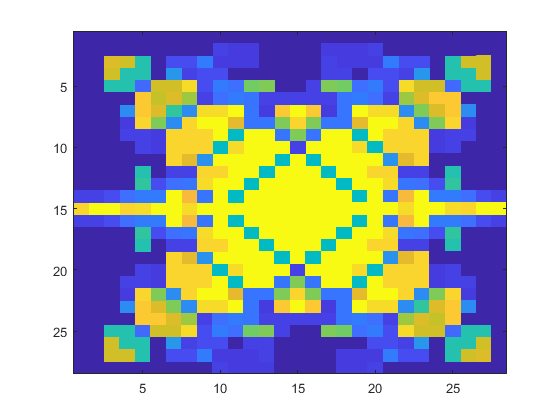
\includegraphics[height=0.4\textheight]{_ref_/kohonen/1}
	\caption{Слой Кохонена ($w_j0 = 0$)\label{fig:01}}
\end{figure}

После прохождения слоя линейных элементов сигналы посылаются на обработку по правилу «победитель забирает всё»: среди выходных сигналов выполняется поиск максимального (либо минимального) $D_j$:
$$ j_{ok} = arg\max_{j}(D_j) $$
или
$$ j_{ok} = arg\min_{j}(D_j) $$
Окончательно, на выходе сигнал с номером $j_{ok}$ равен единице, остальные – нулю. Если же максимум одновременно достигается на нескольких $j_{ok}$, то все соответствующие сигналы принимают равными единице, либо равным единице по соглашению принимается только первый из сигналов в списке. \\

Нейронная сеть Кохонена представляет собой типичный пример нейросетевой архитектуры, обучающейся без учителя. Отсюда и перечень решаемых ими задач: кластеризация данных или прогнозирование свойств. 

Кроме того, сети Кохонена могут использоваться с целью уменьшения размерности данных с минимальной потерей информации. 

В рассматриваемой архитектуре сигнал распространяется от входов к выходам в прямом направлении, как, например, в FFNN-сети. Однако FFNN, как и многие другие архитектуры, обучается с учителем на выборках данных, включающих множество примеров, состоящих из соответствующих друг другу пар входных и выходных векторов. При этом выходные значения принимают самое непосредственное участие в настройке весовых коэффициентов. Так, при выполнении лабораторной работы №1 в системе MATLAB был реализован программный модуль обучения стандартной FFNN-сети (персептрона). Обучение предполагало тренировку сети с помощью метода обратного распространения ошибки на примерах вида 
$$\left(I_j; v_j\right)$$
где $I_j$ — j-e изображение геометрической фигуры, $v_j$ — соответствующий ему вектор-метка.\\
Вектор $v-j$: \emph{треугольник} -- [1, 0, 0, 0, 0]; \emph{квадрат} -- [0, 1, 0, 0, 0]; \emph{круг} -- [0, 0, 1, 0, 0]; \emph{пятиугольник} -- [0, 0, 0, 1, 0];  \emph{шестиугольник} -- [0, 0, 0, 0, 1].

В нейронных сетях Кохонена выходные вектора в обучающей выборке могут быть, но могут и отсутствовать, и, в любом случае, они не принимают участия в процессе обучения. То есть выходы не используются в качестве ориентиров при коррекции синапсов. Именно поэтому данный принцип настройки нейронной сети называется самообучением (обучением без учителя). 

Количество нейронов N делают равным количеству кластеров, среди которых происходит начальное распределение и последующее перераспределение обучающих примеров. Количество входных переменных нейронной сети равно числу признаков, характеризующих объект исследования и на основе которых происходит отнесение его к одному из кластеров.


Рассмотрим геометрическую интерпретацию слоя Кохонена.
Пусть каждому j-му нейрону поставлена в соответствие точка 
$$W_j = (w_{j1}, ..., w_{jM})$$
в M-мерном пространстве. Будем для каждого входного вектора 
$$x = (x_1, ..., x_M)$$
вычислять его расстояния $\rho_{j}(x)$ до точек $W_j$ для каждого нейрона), например, в евклидовой метрике. Примем $\|v\|$ за обозначение евклидовой длины вектора v, тогда:
$$\rho_{j}(x) = \|x-W_j\|^{2} = \|W_j\|^2 - 2
\sum\limits_{i=1}^{M} w_{ji} x_i + \|x\|^{2}$$
Заметим, что последнее слагаемое $\|x\|^{2}$ одинаково для каждого j.

\begin{figure}[h!]
	\centering
	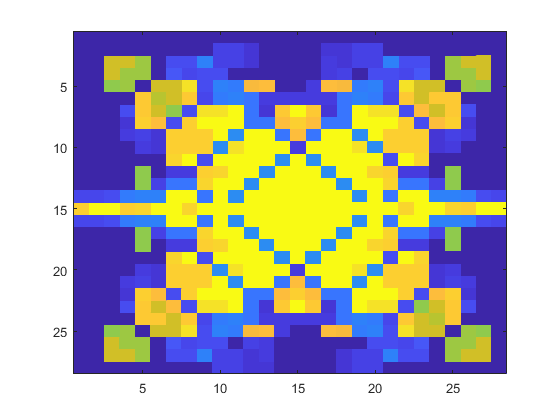
\includegraphics[height=0.2\textheight]{_ref_/kohonen/2}
	\caption{Argmin ($w_{j0} = 0$)\label{fig:02}}
\end{figure}

По принципу «победитель забирает всё» найдём тот нейрон, для которого расстояние до вектора x минимально (argmin) (рис.\,\ref{fig:02}). 

\newpage

\[
j_ok = arg\min_{j}\rho_{j}(x) = arg\min_{j}\left(
\|W_j\|^{2} - 2 \sum\limits_{i=1}^{M} w_{ji} x_i
\right) = 
\]
\[arg\min_{j}\left(
\frac{1}{2}\|W_j\|^{2} - \sum\limits_{i=1}^{M} w_{ji} x_i
\right) = 
arg\min_{j}\left(
- \frac{1}{2}\|W_j\|^{2} + \sum\limits_{i=1}^{M} w_{ji} x_i
\right)
\]
\[ = arg\min_{j}\left(
w_{j0} + \sum\limits_{i=1}^{M} w_{ji} x_i
\right) = arg\min_{j}(D_j)
\]
где $w_{j0} = - \frac{1}{2}\|W_j\|^{2}$


В случае если точки $W_j$ изначально заданы, имеющееся M-мерное пространство разобьется на т.н. многогранники Вороного-Дирихле $V_j$ (рис.\,\ref{fig:02}) Каждый многогранник $V_j$ состоит из точек, которые ближе к $W_j$, чем к другим $W_k$, где $k \neq j$.

\begin{figure}[h!]
	\centering
	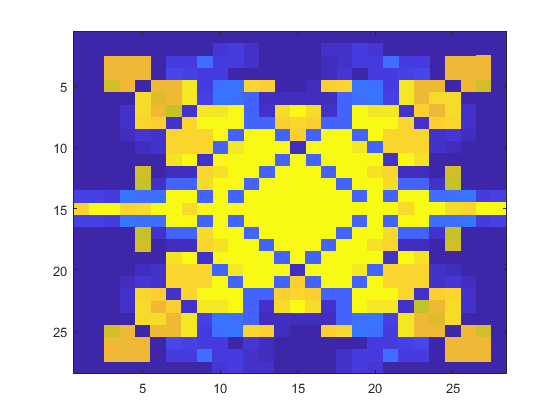
\includegraphics[height=0.4\textheight]{_ref_/kohonen/3}
	\caption{Argmin ($w_j0 = 0$)\label{fig:03}}
\end{figure}

Следует различать собственно самообучение и самоорганизацию нейронной сети Кохонена. При обычном \emph{самообучении} сеть имеет строго фиксированную структуру, т. е. количество нейронов, не изменяющееся на протяжении всего жизненного цикла. \\
При \emph{самоорганизации} сеть, напротив, не имеет постоянной структуры. В зависимости от найденного расстояния до нейрона-победителя либо этот нейрон используется для кластеризации примера, либо для поданного на входы примера создается новый кластер с соответствующими ему весовыми коэффициентами. Кроме того, в процессе самоорганизации структуры сети Кохонена отдельные нейроны могут исключаться из нее.


\section{Описание разработанных ПМ и решение задачи}

Для решения поставленной задачи распознавания геометрических фигур на фоне различных цветов с помощью нейронной сети Кохонена реализуем обучающую и тестовую выборки изображений. В качестве геометрических фигур рассмотрим правильные n–угольники. Для $n = 3$ — треугольник, $n = 4$ — квадрат, $n = 5$ — пятиугольник, $n = 6$ — шестиугольник и $n = 100$ — круг. (рис.\,\ref{fig:04})

\begin{figure}[tbh!]
	\center
	\newdimen\R
	\R=.6cm
	\begin{tikzpicture}
	% Indicate the boundary of the regular polygons
	\draw[fill=red!25] (0:\R) \foreach \x in {120,240} {
		-- (\x:\R)
	} -- cycle (90:\R);
	\draw[fill=green!25,xshift=2.5\R] (0:\R) \foreach \x in {90,180,...,359} {
		-- (\x:\R)
	} -- cycle (90:\R);
	\draw[fill=blue!25,xshift=5.0\R] (0:\R) \foreach \x in {72,144,...,359} {
		-- (\x:\R)
	} -- cycle (90:\R);
	\draw[fill=magenta!25,xshift=7.5\R] (0:\R) \foreach \x in {60,120,...,359} {
		-- (\x:\R)
	}-- cycle (90:\R);
	\draw[fill=black!25,xshift=10.0\R] (0:\R) \foreach \x in {3.6,7.2,...,359} {
		-- (\x:\R)
	} -- cycle (90:\R);
	\end{tikzpicture}
	\caption{N-угольники}
	\label{fig:04}
\end{figure}

Был реализован алгоритм, позволяющий получить изображения указанных геометрических фигур различных размеров и цветов. Предусмотрена возможность поворота фигуры на некоторый случайный угол.

\subsubsection*{Файлы \texttt{Matlab}:}
\verb|gen_set_of_ngons.m|\\
\verb|gen_ngon_image.m|\\
\verb|run_gen_ngon.m|\\[6pt]

Как и в лабораторной работе №1 реализуем 2 выборки: «сложную» и «упрощённую». 

\subsubsection*{Выборка \textnumero\,1 ''Сложная''}
Изображения размером 28×28 пикселей. Фигуры расположены произвольно относительно центра изображения, произведён поворот на случайный угол. Цвет фигуры и цвет фона также случайные.

\begin{figure}[H]
	\centering
	\includegraphics[scale=0.125]{_ref_/3-gone-smpl}	
	\includegraphics[scale=0.125]{_ref_/4-gone-smpl}
	\includegraphics[scale=0.430]{_ref_/5-gone-smpl}	
	\includegraphics[scale=0.125]{_ref_/6-gone-smpl}	
	\includegraphics[scale=0.125]{_ref_/100-gone-smpl}						
	\caption{Примеры сгенерированных фигур}
	\label{fig:05}
\end{figure}

\subsubsection*{Выборка \textnumero\,2 ''Упрощённая''}
Содержит изображения фигур с фиксированными положением, размером и цветом. От изображения к изображению меняется только цвет фона.  Данная выборка представляет собой упрощённый вариант выборки-1.

\subsubsection*{Выборка \textnumero\,2 ''Упрощённая''}
Вариация выборки-2 «упрощённой»: к существующим изображениям добавляются те же, но зашумленные гауссовским шумом до максимального уровня 0.5.

Все изображения переведём в оттенки серого и преобразуем в одномерный массив длиной 784 элемента. 

\subsubsection*{Обучение}
Перед применением к сгенерированным выборкам сети Кохонена, необходимо произвести нормализацию входных переменных, которая может быть выполнена в пределах [–1, 1] или [0, 1]. Выберем первый вариант, так как такая нормализация уже использовалась в лабораторной работе №2 перед применением сети Хопфилда. 

Алгоритм обучения сети Кохонена включает этапы, состав которых зависит от типа структуры: постоянной (самообучающаяся сеть) или переменной (самоорганизующаяся сеть). В данной работе будем рассматривать только самообучающуюся сеть. 


Для самообучения последовательно выполняются:

1.	Задание структуры сети (кол-ва нейронов N в слое Кохонена). 

2.	Случайная инициализация весовых коэффициентов значениями, удовлетворяющими одному из следующих ограничений:\\
a.	При нормализации исходной выборки в пределах [-1, 1]:
$$|w_{ij}| \leq \frac{1}{\sqrt{M}}$$
b.	При нормализации исходной выборки в пределах [0, 1]:
$$0.5 - \frac{1}{\sqrt{M}} \leq w_{ij} \leq 0.5 + \frac{1}{\sqrt{M}}$$
M – количество входных переменных сети.

3.	Подача на входы сети случайного обучающего примера текущей эпохи обучения и расчет евклидовых расстояний от входного вектора до центров всех кластеров:
$$R_j = \sqrt{\sum\limits_{i=1}{M} \left( X_i - w_{ij} \right)}.$$

4.	По наименьшему из значений $R_j$ выбирается нейрон-победитель j, в наибольшей степени близкий по значениям с входным вектором. Для выбранного нейрона (и только для него) выполняется коррекция весовых коэффициентов.
$$w_{ij}^{q+1} = w_{ij}^{q} + v\cdot \left( X_i - w_{ij}^{q} \right) $$
где v - скорость обучения.

5.	Цикл повторяется с шага 3 до выполнения одного или нескольких условий окончания:
\\
– исчерпано заданное предельное количество эпох обучения;\\
– не произошло значимого изменения весовых коэффициентов в пределах заданной точности на протяжении последней эпохи обучения;\\
– исчерпано заданное предельное физическое время обучения.\\


В MATLAB слой Кохонена создается следующим образом:
\begin{verbatim}
net = newc(PR,S,KLR)
\end{verbatim}
здесь PR –[N (кол-во нейронов) x 2] матрица минимальных и максимальных значений входных переменных. В нашем случае это [-1, 1]. S – число нейронов ( = N). KLR – Kohonen learning rate – скорость обучения по Кохонену (стандарт: 0.01).\\


Обучение производится с помощью:
\begin{verbatim}
net = train(net, P);
\end{verbatim}
где P – подготовленная выборка данных.

\subsubsection*{Файлы \texttt{Matlab}:}
\verb|load_dataset.m|\\
\verb|create_n_train_koh.m|\\
\verb|sim.m|\\[6pt]


В предыдущих лабораторных работах была рассмотрена возможность в качестве дополнительной предобработки изображений, перед подачей данных на вход нейронной сети для классификации, применять к имеющимся изображениям геометрических фигур т.н. Фурье-преобразование с целью получения 2D-спектра фигуры (далее совершая сдвиг по нулевой частоте для центрирования). Как показало исследование, при использовании FFNN-сети, процент распознанных фигур, имеющих произвольные площадь, поворот и цвет на изображении («сложные»), резко возрастает, если предварительно рассчитать по данному изображению его 2D-спектр. Однако воссоздать похожие результаты при использовании сети Кохонена не удалось. Процент распознавания на «сложной» выборке всего ~3-4\%. 
Сеть не способна по тем или иным причинам отнести изображения различных (разных) геометрических фигур из данной выборки (№1) к различным (также – разным) кластерам (даже после Фурье-обработки).
На выборке №2, сеть Кохонена, как и предполагалось (как и FFNN, и сеть Хопфилда), выдает оличный процент распознавания, близкий к 100\%.

\begin{figure}[h!]
	\centering
	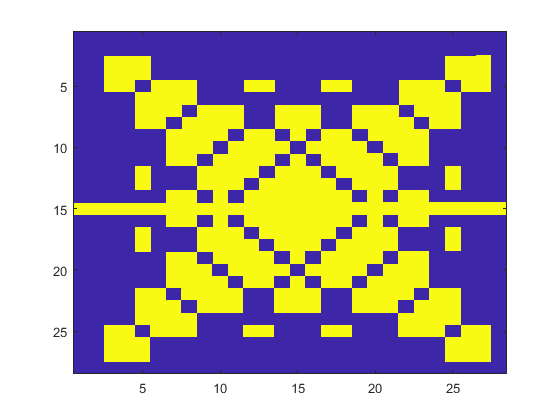
\includegraphics[height=0.4\textheight]{_ref_/kohonen/6}
	\caption{Средства MATLAB. NNtrainTool\label{fig:06}}
\end{figure}

В данный момент автор обучает сеть Кохонена на примерах выборки №3.


\newpage
\section{Альтернативные способы решения}
%Альтернативные способы решения рассматриваемой задачи и сравнение с нейросетевым подходом (отразить достоинства, недостатки, возможные ограничения на постановку задачи и требования по априорной информации для формирования обучающих примеров).
Альтернативными являются два подхода классификации фигур, которые во многом противоположны друг другу.\\
\noindent
\textbf{Первым подходом} является подход на основе спектрального анализа \cite{direkoglu2011}. 
Представление формы объекта на основе \emph{Фурье дескрипторов} легко организовать в плане вычислений,
а результаты будут устойчивы к внешнему шуму. Фурье дескрипторы получаются при помощи преобразования
Фурье, применённого к \emph{сигнатуре формы объекта}, границе объекта как одномерной функции.


\begin{figure}[tbh!]
	\center
	\includegraphics[scale=0.5]{_ref_/direkoglu2011_fig}
	\caption{Пример обработки изображения лошади \cite{direkoglu2011}}
	%	\label{fig:08}
\end{figure}
Существуют и другие сигнатуры формы, например, расстояние от центра объекта (в пикселях) до остальных пикселей,
кривизна границы и кумулятивный угол. Геометрические характеристики (инварианты) объекта
определяются на этапе определения сигнатуры формы объекта, который может происходить как до
Фурье преобразования, так и после. При этом, нижние частоты дескрипторов содержат
информацию о форме объекта, а верхние частоты о деталях.

\noindent
\textbf{Вторым подходом} является геометрический подход, который предполагает выделение контура \cite{wang2014}. 
Он основывается на разработке дескрипторов формы малого разрешения, которые могут быть
устойчивы к поворотам, масштабированию и деформации объекта.

\begin{figure}[H]
	\center
	\includegraphics[scale=0.44]{_ref_/xinggang2014_fig}
	\caption{Пример обработки изображения бабочки \cite{wang2014}}
	%	\label{fig:08}
\end{figure}

В таком подходе граница объекта разбивается на составные части (сегменты), каждая
из которых далее описывается при помощи того или иного дескриптора. После чего
для решения задачи классификации применяются методы машинного обучения, например,
метод опорных векторов \cite{svm}.


\section{Области применения НС заданного типа}
Сети финского ученого Кохонена применяются для решения самых разнообразных задач моделирования и прогнозирования, выявления наборов независимых признаков, поиска закономерностей в больших массивах данных, разработке компьютерных игр, квантизации цветов к их ограниченному числу индексов в цветовой палитре: при печати на принтере и ранее на ПК или же на приставках с дисплеем с пониженным числом цветов, для архиваторов или видео-кодеков, и т. д. 


\newpage
\appendix 

\addcontentsline{toc}{section}{Список литературы}


\begin{thebibliography}{99}
\bibitem{xxx}  Kohonen, T. (1989/1997/2001), Self-Organizing Maps, Berlin — New York: Springer-Verlag. First edition 1989, second edition 1997, third extended edition 2001, ISBN 0-387-51387-6, ISBN 3-540-67921-9

\bibitem{kkk} Hecht-Nielsen, R. (1990), Neurocomputing, Reading, MA: Addison-Wesley, ISBN 0-201-09355-3.

\bibitem{cohen1983} Cohen M.A., Grossberg S.G., Absolute stability of global pattern formation and parallel memory storage by compatitive neural networks. IEEE Transactions on Systems, Man and Cybernetics, Vol. 13, 1983, pp. 815--26. \textbf{DOI:~:10.1109/TSMC.1983.6313075}
%
%\bibitem{NNzoo} Шпаргалка по разновидностям нейронных сетей. Часть первая. Элементарные конфигурации. \textbf{URL:~\url{https://tproger.ru/translations/neural-network-zoo-1/}}
%
%\bibitem{FFNNsample} A simple example of feedforward neural network and image recognition.
%\textbf{URL:~\url{https://dummas.wordpress.com/2012/01/14/a-simple-example-of-feedforward-neural-network-with-image-recognition/}}

\bibitem{hou1999} Tung-Hsu Hou and Ming-Der Pern, A Computer Vision-Based Shape-Classification System Using
Image Projection and a Neural Network.
Int. J. Adv. Manuf. Technol., 15, 1999, pp. 843--850.
\textbf{DOI:~10.1007/s001700050141}

\bibitem{direkoglu2011} Cem Direko\u{g}lu, Mark S. Nixon, Shape classification via image-based multiscale description.
Pattern Recognition, 44, 2011, pp. 2134--2146. \textbf{DOI:~10.1016/j.patcog.2011.02.016}

\bibitem{wang2014} Xinggang Wang, Bin Feng, et.al., Bag of contour fragments for robust shape classification.
Pattern Recognition, 47, 2014, pp. 2116--2125. \textbf{DOI:~10.1016/j.patcog.2013.12.008}

\bibitem{svm} К.В. Воронцов. Лекции по методу опорных векторов. \textbf{URL:~\url{http://www.ccas.ru/voron/download/SVM.pdf}}

\end{thebibliography}


\newpage
\appendix 
\addcontentsline{toc}{section}{Тексты программ}

\section*{Тексты программ}

\verb|gen_ngon_image.m|
\begin{lstlisting}
function out = gen_ngon_image(n)

%% Suppose that domain is [0 100]x[0 100] square
dom = [0 100 0 100];

% Center of n-polygon
xC = randi([30 70],1,1);
yC = randi([30 70],1,1);
center = [xC yC];
nS = n; % number of sides of n-gon
th = linspace(0, 2*pi, nS + 1);
% Rotate the shape by subtracting an offset.
rot = randi([-10 10],1,1);
th = th - pi/rot;
R = randi([15 35],1,1);
x = R * cos(th) + center(1);
y = R * sin(th) + center(1);

%% Show image
figure_color        = 0.5 + 0.5*rand(1,3);
background_color    = 0.2*rand(1,3);

h = fill(x, y, figure_color);
set(h,'edgecolor',figure_color);
ax = gca;
set(ax,'xtick',[]); set(ax,'ytick',[]);

ax.XColor = background_color; ax.YColor = background_color ;
axis square; axis(dom);
set(ax,'Color',background_color )

img = getframe(gca);
out = img;
\end{lstlisting}

\noindent
\verb|gen_set_of_ngons.m|
\begin{lstlisting}
function gen_set_of_ngons(number_of_images, nS, folder, baseFileName, type, speedup)

if strcmp(type,'simplified')
if strcmp(speedup,'yes')
parfor k = 1:number_of_images
img = gen_ngon_image_simplified(nS);
fullFileName = [folder  baseFileName '-' int2str(k)  '.png'];
save_image(folder,baseFileName,fullFileName,img.cdata);
disp([int2str(k) '/' int2str(number_of_images)])
end %for k
else
for k = 1:number_of_images
img = gen_ngon_image_simplified(nS);
fullFileName = [folder  baseFileName '-' int2str(k)  '.png'];
save_image(folder,baseFileName,fullFileName,img.cdata);
disp([int2str(k) '/' int2str(number_of_images)])
end %for k
end %if
else
if strcmp(speedup,'yes')
parfor k = 1:number_of_images
img = gen_ngon_image(nS);
fullFileName = [folder  baseFileName '-' int2str(k)  '.png'];
save_image(folder,baseFileName,fullFileName,img.cdata);
disp([int2str(k) '/' int2str(number_of_images)])
end %for k
else
for k = 1:number_of_images
img = gen_ngon_image(nS);
fullFileName = [folder  baseFileName '-' int2str(k)  '.png'];
save_image(folder,baseFileName,fullFileName,img.cdata);
disp([int2str(k) '/' int2str(number_of_images)])
end %for k
end %if    
end 
\end{lstlisting}

\noindent
\verb|run_gen_ngons.m|
\begin{lstlisting}
clear all; close all; clc;

% Get path
CurrentFolder = pwd;


% Generate ngon image
number_of_images = 20000;

% Generate set of 3-gons
nS = 100;
type = 'simplified';
speedup = 'yes';
folder = [CurrentFolder '\_img_\' int2str(nS) '-gone-' type '\'];
mkdir_if_not_exist(folder);
baseFileName = [int2str(nS) '-gone'];
gen_set_of_ngons(number_of_images, nS, folder, baseFileName, type, speedup);
% Compress folder with images
zippedfiles = zip([CurrentFolder '\_img_\' int2str(nS) '-gone-' type '.zip'], folder);
% Remove folder with images
rmdir(['_img_/' int2str(nS) '-gone-' type],'s')
\end{lstlisting}

\noindent
\verb|load_dataset.m|
\begin{lstlisting}
triangleFolder = '_img_/3-gone/';       % label: 1
rectangleFolder = '_img_/4-gone/';      % label: 2
circleFolder = '_img_/100-gone/';       % label: 3
pentagonFolder = '_img_/5-gone/';       % label: 4
hexagonFolder = '_img_/6-gone/';        % label: 5

% getting filelists 
dirData = dir(triangleFolder);
dirIndex = [dirData.isdir];
fileListTriangles = {dirData(~dirIndex).name}';
dirData = dir(rectangleFolder);
dirIndex = [dirData.isdir];
fileListRectangles = {dirData(~dirIndex).name}';
dirData = dir(circleFolder);
dirIndex = [dirData.isdir];
fileListCircles = {dirData(~dirIndex).name}';
dirData = dir(pentagonFolder);
dirIndex = [dirData.isdir];
fileListPentagones = {dirData(~dirIndex).name}';
dirData = dir(hexagonFolder);
dirIndex = [dirData.isdir];
fileListHexagones = {dirData(~dirIndex).name}';

N = 1;
hvP_size = 28;
P_size = hvP_size * hvP_size;

trianglesI = zeros(P_size, N);
rectanglesI = zeros(P_size, N);
circlesI = zeros(P_size, N);
pentagonesI = zeros(P_size, N);
hexagonesI = zeros(P_size, N);
trianglesFFT = zeros(P_size, N);
rectanglesFFT = zeros(P_size, N);
circlesFFT = zeros(P_size, N);
pentagonesFFT = zeros(P_size, N);
hexagonesFFT = zeros(P_size, N);

for i = 1:N
fpath = strcat(triangleFolder, fileListTriangles{i});
disp(fpath);
I = imread(fpath);
I = imresize(I, [hvP_size hvP_size]);
II = reshape(I(:,:,1), [P_size, 1]);    
trianglesI(:, i) = II;
I = fft2(I);
I = reshape(abs(fftshift(I(:,:,1))), [P_size,1]);
trianglesFFT(:, i) = I;

fpath = strcat(rectangleFolder, fileListRectangles{i});
disp(fpath);
I = imread(fpath);
I = imresize(I, [hvP_size hvP_size]);
II = reshape(I(:,:,1), [P_size, 1]);
rectanglesI(:, i) = II;
I = fft2(I);
I = reshape(abs(fftshift(I(:,:,1))), [P_size,1]);
rectanglesFFT(:, i) = I;

fpath = strcat(circleFolder, fileListCircles{i});
disp(fpath);
I = imread(fpath);
I = imresize(I, [hvP_size hvP_size]);
II = reshape(I(:,:,1), [P_size, 1]);
circlesI(:, i) = II;
I = fft2(I);
I = reshape(abs(fftshift(I(:,:,1))), [P_size,1]);
circlesFFT(:, i) = I;

fpath = strcat(pentagonFolder, fileListPentagones{i});
disp(fpath);
I = imread(fpath);
I = imresize(I, [hvP_size hvP_size]);
II = reshape(I(:,:,1), [P_size, 1]);
pentagonesI(:, i) = II;
I = fft2(I);
I = reshape(abs(fftshift(I(:,:,1))), [P_size,1]);
pentagonesFFT(:, i) = I;

fpath = strcat(hexagonFolder, fileListHexagones{i});
disp(fpath);
I = imread(fpath);
I = imresize(I, [hvP_size hvP_size]);
II = reshape(I(:,:,1), [P_size, 1]);
hexagonesI(:, i) = II;
I = fft2(I);
I = reshape(abs(fftshift(I(:,:,1))), [P_size,1]);
hexagonesFFT(:, i) = I;
end

N5 = 5 * N;
DataSet_Images_Total = zeros(1, P_size, N5);
DataSet_FFTs_Total = zeros(1, P_size, N5);

% Total
k = 1;
for i = 1:N
DataSet_Images_Total(1,:,k) = trianglesI(:, i);
DataSet_FFTs_Total(1,:,k) = trianglesFFT(:, i);
k = k + 1;

DataSet_Images_Total(1,:,k) = rectanglesI(:, i);
DataSet_FFTs_Total(1,:,k) = rectanglesFFT(:, i);
k = k + 1;

DataSet_Images_Total(1,:,k) = circlesI(:, i);
DataSet_FFTs_Total(1,:,k) = circlesFFT(:, i);
k = k + 1;

DataSet_Images_Total(1,:,k) = pentagonesI(:, i);
DataSet_FFTs_Total(1,:,k) = pentagonesFFT(:, i);
k = k + 1;

DataSet_Images_Total(1,:,k) = hexagonesI(:, i);
DataSet_FFTs_Total(1,:,k) = hexagonesFFT(:, i);
k = k + 1;
end

Images = squeeze(DataSet_Images_Total(1, :, :));
FFTs = squeeze(DataSet_FFTs_Total(1, :, :));
for i = 1:P_size
for j = 1:N5
Images(i, j) = round(Images(i, j)/256);
if (Images(i, j) == 0)
Images(i, j) = -1;
end
if (Images(i, j) > 1)
Images(i, j) = 1;
end
FFTs(i, j) = round(FFTs(i, j)/256);
if (FFTs(i, j) == 0)
FFTs(i, j) = -1;
end
if (FFTs(i, j) > 1)
FFTs(i, j) = 1;
end
end
end

I = reshape(Images(:, 5), [hvP_size, hvP_size]);
imagesc(I);
% I = reshape(FFTs(:, 5), [hvP_size, hvP_size]);
% imagesc(I);
\end{lstlisting}

\noindent
\verb|create_n_train_koh.m|
\begin{lstlisting}
L = zeros(784, 2);
L(:, 2) = ones(784, 1);
% 
net = newc(L, 5);

P = squeeze(DataSet_Images_Total(1, :, :));
% P = squeeze(DataSet_FFTs_Total(1, :, :));

% L = zeros(112, 2);
% L(:, 2) = ones(112, 1);

% net = newc(L, 5);
% 
% P = squeeze(DataSet_Features_Total(1, :, :));


net = train(net, P);
\end{lstlisting}

\noindent
\verb|sim.m|
\begin{lstlisting}
Y = sim(net, P);
Yc = vec2ind(Y);

disp(Yc);
\end{lstlisting}


\newpage
%% Оглавление
\newpage
\tableofcontents

\end{document}